
%(BEGIN_QUESTION)
% Copyright 2015, Tony R. Kuphaldt, released under the Creative Commons Attribution License (v 1.0)
% This means you may do almost anything with this work of mine, so long as you give me proper credit

Analyze the operation of this pneumatic mechanism, identifying whether you think it is {\it force-balance} or {\it motion-balance} in nature:

$$\includegraphics[width=15.5cm]{i00880x01.eps}$$

\vskip 20pt \vbox{\hrule \hbox{\strut \vrule{} {\bf Suggestions for Socratic discussion} \vrule} \hrule}

\begin{itemize}
\item{} Explain how an {\it O-ring seal} functions, based on its representation in this diagram.  What, exactly, is it sealing?  Does it permit motion, or it is a stationary component?
\item{} A powerful problem-solving technique is performing a {\it thought experiment} where you mentally simulate the response of a system to some imagined set of conditions.  Describe a useful ``thought experiment'' for this system, and how the results of that thought experiment are helpful to answering the question.
\item{} Identify how you could alter the {\it bias} (or {\it zero}) of this pneumatic mechanism.  What components, if any, would need to be replaced?
\item{} Identify how you could alter the {\it gain} (or {\it span}) of this pneumatic mechanism.  What components, if any, would need to be replaced?
\end{itemize}

\underbar{file i00880}
%(END_QUESTION)





%(BEGIN_ANSWER)

Half of this mechanism is motion-balance, and the other half is force-balance!

%(END_ANSWER)





%(BEGIN_NOTES)

All components to the right of the spring are motion-balance, while all components to the left of the spring are force-balance.  Students should run ``thought experiments'' on this mechanism to determine its operation.

%INDEX% Measurement, pressure: motion- versus force-balance

%(END_NOTES)


